\chapter{Theory}\label{c:Theory}

\section{Standard Model}


The Standard Model (SM) of particle physics is a collection of several theories which provide the most accurate theoretical framework for describing all known components of matter and their interactions to date. The model describes three fundamental forces, each mediated by an integer spin particle called a \textit{gauge boson}, that control interactions between the spin-$\frac{1}{2}$ \textit{quarks} and \textit{leptons} that make up matter. The mathematical structure is  based on the symmetry group $SU(3)_c\times SU(2)_L\times U(1)_\gamma$ and is required to be gauge-invariant. The SM does not include gravity; gravity cannot be written in the Quantum Field Theories that describe the Standard Model, and gravitational interactions are significantly weaker than the other fundamental forces (Table \ref{t:tab:boson}). As a result, gravitational interactions so are neglected hereafter.

	\subsection{Fermions}

		The full set of spin-$\frac{1}{2}$ \textit{fermions}, described in Tables \ref{t:tab:quark} and \ref{t:tab:lepton}, are the quark and lepton families, which each have three generations. For each distinct particle there is a paired \textit{anti-particle} which is identical aside from opposite charge and \textit{handedness}.

		The handedness or helicity of a particle refers to the projection of the angular momentum of the particle along the direction of the particle momentum. For a spin $\frac{1}{2}$ particle, the angular momentum component can be aligned along the direction of motion (\textit{positive} or \textit{right-handed} alignment) or opposed to it (\textit{negative} or \textit{left-handed} alignment)). This

		Most matter consists of the observable first generation of the up and down quarks and the electron which make up protons and neutrons, along with the unobservable electron neutrino. Both the leptons and the quarks obey Fermi-Dirac statistics. Quarks experience all three fundamental forces, charged leptons interacting via the electromagnetic and weak interactions and neutral leptons experiencing only the weak interaction.

		{
		\setlength{\extrarowheight}{5pt}
		\begin{table}[ht]
			\caption{Spin-$\frac{1}{2}$ fermions: quarks $q$ \cite{pdg}. The top quark mass is taken from direct measurements.}
			\label{t:tab:quark}
			\medskip
			\centering
			\begin{tabular}{clcc}\toprule
				Generation & Flavour & Charge / $e$ & Mass / GeV \\\midrule
				1    &     Up $u$      &    +2/3   & $0.0022\ _{-0.0004}^{+0.0006}$\\
	    &     Down $d$    &    -1/3   & $0.0047\ _{-0.0004}^{+0.0005}$\\
		    	2    &     Charm $c$      &    +2/3   & $1.28\pm0.03$\\
		    	&     Strange $s$    &    -1/3   & $0.096\ _{-0.004}^{+0.008}$\\
				3    &     Top $t$  &   +2/3   & $173.1\pm0.6$\\
	    &     Bottom $b$   &   -1/3   & $4.18\ _{-0.03}^{+0.04}$\\\bottomrule
			\end{tabular}\\[5pt]
		\end{table}
		}
		\begin{table}[ht]
			\caption{Spin-$\frac{1}{2}$ fermions: leptons $l$ \cite{pdg}}
			\label{t:tab:lepton}
			\medskip
			\centering
			\begin{tabular}{clcl}\toprule
				Generation & Flavour & Charge / $e$ & Mass / MeV\\\midrule
				1    &     Electron $e$      &    -1   & $0.5109989461\pm0.0000000031$\\
				&     Electron Neutrino $\nu_e$    &   0  & $<2\times10^{-6}$ \\
				2    &     Muon $\mu$      &    -1   & $105.6583745\pm0.0000024$\\
				&     Muon Neutrino $\nu_\mu$    &    0   & $<2\times10^{-6}$ \\
				3    &     Tau $\tau$  &   -1   & $1776.86\pm0.12$\\
				&     Tau Neutrino $\nu_\tau$   &   0   & $<2\times10^{-6}$ \\\bottomrule
			\end{tabular}\\[5pt]
		\end{table}

		Quarks are always confined into colour singlet \textit{hadrons} bound by the strong interaction, which are either \textit{baryons} ($qqq$) like the \textit{proton} ($uud$) and \textit{neutron} ($ddu$), or \textit{mesons} ($q\bar{q}$) like the positive \textit{pion} ($u\bar{d}$). }.

	\subsection{Forces}

		All forces arise due the exchange of unobservable virtual particles, gauge bosons, which obey Bose-Einstein statistics. The three fundamental particle interactive forces for the SM are named the strong, weak and electromagnetic interactions, and are mediated by \textit{gluons}, \textit{weak bosons} and \textit{photons} respectively. The gauge bosons are described in more detail in Table \ref{t:tab:boson}.

		\begin{table}[ht]
			\caption{Spin-1 gauge bosons. The strength of the interaction is typically stated in terms of $\alpha$, a dimensionless constant proportional to the matrix element for the virtual particle exchange for each interaction. For the  The weak interaction is intrinsically stronger than the EM interaction, but the mass of the weak bosons limits the range to extremely short distances.  The strength of gravity is $\sim10^{-39}$ hence it is neglected. \cite{pdg}}
			\label{t:tab:boson}
			\medskip
			\centering
			\begin{tabular}{clclc}\toprule
				Interaction & Particle & Charge / $e$ & Mass / GeV & Strength ($\alpha$) \\\midrule
				Strong    &     Gluon $g$      & 0 & 0 & $\sim1$\\
				Weak (Charged Current)&     $W^+$    &    1   & $80.385\pm0.015$ & \\
				&     $W^-$    &    -1   & $80.385\pm0.015$ & $10^{-6}$ \\
				Weak (Neutral Current)&     $Z$   &    0   & $91.1876\pm0.0021$ & \\
				Electromagnetic (EM)   &     Photon $\gamma$  &  $<1\times10^{-35}$   & $<1\times10^{-27}$ & $\frac{1}{137}$\\\bottomrule
			\end{tabular}\\[5pt]
		\end{table}

		\newpage
		\subsubsection{Quantum Chromodynamics}

		Quantum Chromodynamics (QCD) is the theory of the strong interaction, mediated by the gluon which couples to colour charge. It corresponds to the $SU(3)_c$ symmetry group of the overall SM. The strong interaction conserves energy, momentum, angular momentum and colour charge. Only quarks and gluons themselves possess colour charge, so while quarks are the only fermion to feel the strong interaction, gluons can self-couple.

		\subsubsection{Electroweak Unification}

		Electroweak Unification (EW) is the expression of the electromagnetic interaction and the weak interaction as separate manifestations of a combined electroweak force in the Glashow-Weinberg-Salam model \cite{gws-g, gws-w, gws-s}, which corresponds to the $SU(2)_L\times U(1)_\gamma$ symmetry group. Quantum Electrodynamics (QED) describes the macroscopically observable $U(1)$ electromagnetic force  with the photon as the mediating boson, and any interaction conserves energy, momentum, parity and charge and additionally never changes particle type through the interaction. The $SU(2)$ weak interaction is mediated by the charged current vector bosons $W^+$, $W^-$ and the neutral current vector boson $Z$, which have large masses that limit the weak interaction to very short distances. The charged current interaction is capable of changing the flavour of a particle and also of violating parity in an interaction.

		The weak interaction by itself was observed to diverge from observation at high energies, leading to the introduction of the unified theory. The combined  $SU(2)_L\times U(1)_\gamma$ group produces four gauge bosons which mix to produce the more recognisable $\gamma$, $W^+$, $W^-$  and $Z$ bosons. The unified force couples to weak isospin, which allows self-coupling between the massive vector bosons, but not the photon as it does not carry electric charge.

		While the weak interaction acts on both quarks and leptons, the quark sector is affected by the distinction between the mass and flavour eigenstates of quarks. The physically observed flavour eigenstates are distinct from the quark eigenstates of the weak interactions, which are superpositions of the mass eigenstates. The effect of this quark mixing in the weak interaction is that different flavour changing interactions have different strengths. The mixing of the mass eigenstates ($q$) into weak eigenstates ($q^\prime$) is described by the Cabbibo-Kobayashi-Makasawa matrix \cite{ckm-c, ckm-km}:

		\begin{equation}
		\begin{pmatrix}
		d^\prime \\
		s^\prime\\
		b^\prime \\
		\end{pmatrix}
		 = \begin{pmatrix}
		V_{ud} & V_{us} & V_{ub} \\
		V_{cd} & V_{cs} & V_{cb} \\
		V_{td} & V_{ts} & V_{tb} \\
		\end{pmatrix}
	    \begin{pmatrix}
	    d \\
	    s\\
	    b \\
	    \end{pmatrix}
		\end{equation}



	\subsection{Spontaneous Symmetry Breaking: The Higgs Boson}
	\label{t:symbreak}


	In addition to the forces, particles acquire mass by coupling to the \textit{Higgs} field via the spin-$0$ Higgs boson \cite{gauge-boson-mass, higgs-1, higgs-2}, which is covered in more detail in Section \ref{t:symbreak}.

	OUT OF PLACE

	The gauge field theories used for the QCD and EW models when unaltered require massless gauge bosons in order to preserve gauge invariance, which follows from the Klein-Gordon equation:
	\begin{equation}
		\frac{\partial^2\psi}{\partial t^2} = (\nabla^2 - m^2)\psi
	\end{equation}
	 This is satisfactory for the gluon and photon, but a separate theory is required to explain the mass of the $W^\pm$ and $Z$ bosons. The Higgs Mechanism proposed introducing a scalar field that interacts with the $W^\pm$ and $Z$ fields. In the Lagrangian formulation this results in a term akin to a mass term ($\propto\psi^2$) which effectively links that mass of the bosons to their coupling with this scalar field. This addition to the Lagrangian is still required to preserve the symmetry of the system and respect the gauge invariance, but is also required to have a non-zero expectation value for the field in the vacuum or ground state of space. The Higgs mechanism introduces the scalar field $\phi$ which has a potential energy $V(\phi)$:
	 \begin{equation}
		 V(\phi) = a\phi^4 - b\phi^2
	 \end{equation}

	This results in an equilibrium point ($\phi=0$) that respects the symmetry, but is inherently unstable, with an infinite set of degenerate non-zero minima at $|\phi^2|=\frac{b}{2a}$ where the symmetry is \textit{spontaneously} broken. This field, in an analogous fashion to the other quantum fields of the SM, can produce particles from excitations which form the physical \textit{Higgs Scalar Boson} $H$. Confirmation of the Higgs boson as part of the SM was only achieved relatively recently \cite{higgs-atlas, higgs-cms}, where a spin-$0$ boson consistent with the SM Higgs was observed. Subsequent measurements made have provided agreement on the new particle as the Higgs boson with a mass of $125.09$\,GeV \cite{pdg}. Section \ref{t:higgs} covers in more detail the production and behaviour of the Higgs boson in collider experiments.


\section{Physics of \textit{pp} Collisions}

	Recent experimental efforts to probe the Standard Model have focused on high-energy collider experiments, where beams of particle with equal energy are collided head on within detectors.  For proton-proton ($pp$) collisions, matters are complicated as the colliding protons are composite particles, which at high energy consist of the three \textit{valence} quarks and a sea of virtual quarks and gluons. Collectively these constituents are referred to as \textit{partons} where each parton carries a fraction of the overall hadron momentum, and the interaction in the $pp$ collision consists of elastic scattering between these partons. At a given energy scale $Q^2$ the probability that a parton $i$ carries a fraction $x_i$ of the overall momentum is described by the parton distribution function (PDF) $f_i(x, Q^2$). These PDFs cannot be calculated from QCD but can be determined from experimental measurements, and collections of PDFs have been assembled from the leading collider experiments \cite{pdfs}.

	In any particle interaction, the probability a particular reaction occurs is in proportion to the cross section of the reaction. The cross section for a short range, hard parton-parton collision is given by $\hat{\sigma}(Q^2)$, where scattering energy scale $Q^2 = x_1x_2E^2_{cm}$ in the parton-parton centre-of-mass frame where $E_{cm}$ is the energy in the centre-of-mass frame. To compute the cross section $\sigma$ for some hard process $pp\rightarrow X$, all possible combinations of incoming partons must be summed over and the momentum fractions integrated over while accounting for the PDFs:
	\begin{equation}
	\sigma = \sum_{i, j = q, g} \int dx_1dx_2f_i(x_1, Q^2)f_j(x_2, Q^2)\hat{\sigma}(Q^2)
	\end{equation}

	\subsection{Geometry}
	\label{t:geometry}

	The high energy protons used in collisions are relativistic in nature, and as the momenta of the colliding partons are not guaranteed to be equal and opposing there is always an unknown element of longitudinal boosting in $pp$ collisions. As a consequence, use of light-cone coordinates and some definitions of convenient quanties can be of benefit to $pp$ collision analyses \cite{lightcone-all-that}.

	Typically the momentum in the transverse plane \pt is used for a particle, and the rapidity $y$ of a particle with non-zero \pt is defined:
	\begin{equation}
	y = \frac{1}{2}\ln\frac{E+p_z}{E- p_z}
	\end{equation}

	This rapidity $y$ transforms additively to boosts along the $z$ axis, so any rapidity difference between two objects is invariant to such boosts. For cases where the mass of a particle is negligible (highly relativistic particles) the rapidity can be related to the polar angle of the particle as the pseudo-rapidity $\eta$:
	\begin{equation}
	\eta = -\ln\tan\frac{\theta}{2}
	\end{equation}

	The distance between two objects within the detector is commonly expressed in the ($\eta$, $\phi$) space rather than absolute, with this separation being given by $\Delta R = \sqrt((\Delta\eta)^2 + (\Delta\phi)^2)$

	\subsection{Collision simulation}

	A $pp$ collision is a complex event which results if a significant number ($\mathcal{O}(1000)$) of final state particles, each of which interact and evolve over the timescale of an event. This progression of the collision event can be broken down into distinct stages of behaviour of the produced particles: the \textit{hard process}, \textit{parton shower}, \textit{hadronisation}, \textit{unstable particle decays} and \textit{underlying event}.

	This breakdown is key to the simulation of $pp$ collisions using Monte-Carlo event generators, the use of which is critical in current high energy physics research. Monte-Carlo simulations of collisions are used to predict and prepare for real data-taking experiments, obtain control datasets of particular particle interactions and act as controls to optimise analysis tools. The breakdown of the interaction into distinct stages has allowed specialised software to be produced for each step, which makes use of a characteristic scale and certain safe approximations for the step to provide reliable predictions, while reducing the computational demands of the simulation \cite{monte-carlo}.

		\subsubsection{Hard Process}

			The first stage of a $pp$ collision and the first step of a simulation, the hard scatter refers to highest momentum transfer process in the event between coloured particles, and forms the core of the event. This details the interaction of partons entering the event and those outgoing partons resulting from the process. In simulation the probability distribution of the partons is calculated from perturbation theory to the desired accuracy (LO, NLO etc) using the PDFs of the constituents.

		\subsubsection{Parton Shower}

			While the hard scatter interaction in a collision is relatively straightforward, the overall behaviour of the partons is much more complex as they progress through the event. The incoming and outgoing partons from the hard scatter radiate additional interaction particles during the event
			The Bremsstrahlung  radiation of photons by scattered electric charges is well described by QED, and the analogous radiation of gluons by scattered colour charges as explained by QCD produces additional partons within the interaction. However, as the gluons produced by QCD scattering themselves carry colour charge, there is extending showering of gluons producing gluons, resulting in the phase space of the interaction being filled with a sea of soft gluons. Both of these radiative processes make up the parton shower stage of the event simulation.

			The evolution of these parton showers is evaluated in Monte-Carlo simulations using a step-by-step iterative process, on the scale of momentum transfer in the interaction. This process is started at the hard scatter and evolved through the interaction with decreasing momentum scale until the point at which perturbation theory breaks down, necessitating a different evaluation method.

		\subsubsection{Hadronisation}
		\label{t:hadronisation}

			With the breakdown of perturbation theory at low momentum scales,  observable colourless hadrons are constructed from the coloured partons using hadronisation models in order to extend the simulation. These hadrons are the physical final state particles observed in the detector, which exist due to the colour confinement of the quarks and gluons. Within a particle detector, rather than individual hadrons \textit{jets} of hadrons are observed. As a coloured fragment produced in the interaction moves away from the interaction, it will create other coloured fragments around itself in order to produce a confined hadron while moving away from the collision. This occurs repeatedly for each hadron ejected from the collision as it moves away, producing a collimated stream of hadrons which make up a jet.

			In simulation this step involves collecting the partons produced in the parton shower into hadrons, and is typically evaluated using either a String model \cite{stringmodel} or a Cluster model \cite{clustermodel}. These steps are models, and not calculations as to how the partons combine, as to calculations being prohibited by the breakdown of perturbation theory.

		\subsubsection{Unstable Particle Decays}

			The final stage of the evolution of the parton shower considers the hadrons produced during the shower. These hadrons may not be stable particles but could be resonances that go on to decay within the detector to produce the more stable hadrons observed in the data. Most modern simulation software models these decays, but the exact specification of the decay tables and channels has a significant impact on the final state of the simulation.

		\subsubsection{Underlying Event}
		\label{t:underlying}

			While the hard scatter and subsequent parton shower results from the highest momentum interaction of the $pp$ collision, the remnants of the proton not involved in this will continue to interact with each other. This produces additional soft hadrons that fill the interaction environment, overlapping with the products of the hard scatter interaction.

			The dominant model for simulation of the underlying event is a perturbative model where the other components undergo additional discrete hard scatter interactions and corresponding parton showers which are simulated in an corresponding fashion to the core scattering.

	\subsection{Monte-Carlo Software}

		There is a broad selection of software tools for evaluating $pp$ collisions, from general purpose simulations like \textsc{Pythia}\cite{pythia} or \textsc{Sherpa}\cite{sherpa} which are used to evaluate the complete process, to more specific tools like \textsc{Powheg}\cite{powheg} which is used to produce hard scatter events with NLO matrix elements. Most software packages make use of the chain of generation for an event outlined previously, and modern analyses will make use of multiple generators interfaced together to compute different steps with improved accuracy.

\section{The Higgs Boson}
\label{t:higgs}

	Detecting the SM Higgs boson is strongly dependent on the predominant production and decay channels for the Higgs boson, which in turn depend on the specifications of the collider used for the search. In this section the relevant production and decay channels at the Large Hadron Collider (LHC) will be discussed.

			\begin{figure}[h]
				\centering
				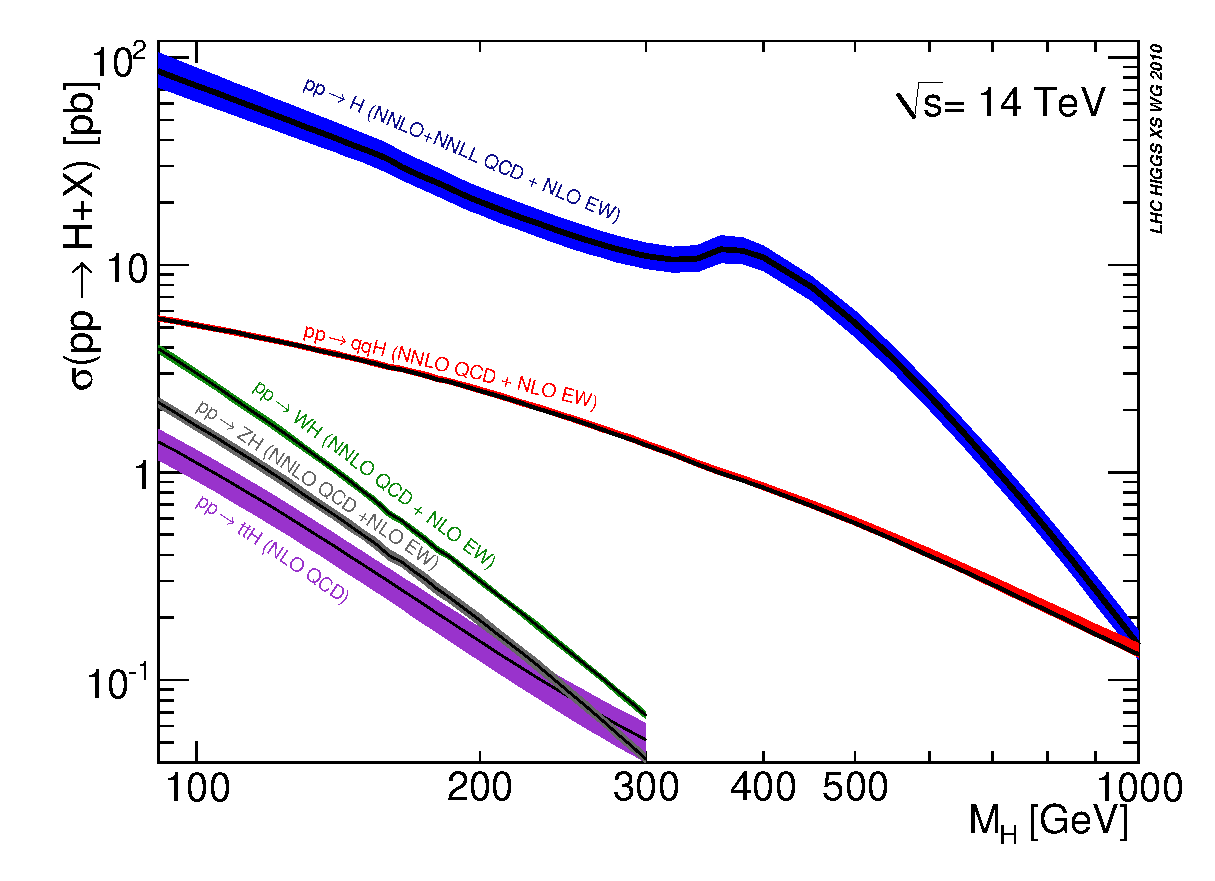
\includegraphics[width=0.7\linewidth]{T/FIGS/YRHXS_Summary_fig3}
				\caption{SM Higgs Production cross section for $\sqrt{s}=14$ TeV. $\,pp\rightarrow H$ corresponds to gluon-gluon fusion production and $pp\rightarrow qqH$ vector boson fusion. \cite{LHCHiggsCS}}
				\label{fig:higgsproductionCS}
			\end{figure}

	\subsection{Higgs Production}

		While there are many various methods for production of a Higgs boson, at the LHC the cross section is dominated by gluon-gluon fusion (\ggF) as shown in Figure \ref{fig:higgsproductionCS}, with the second largest cross-section arising from Vector Boson Fusion (VBF, Section \ref{t:VBF}). Other significant production processes are the associated production with a weak boson ($WH/ZH$, Higgs-strahlung) production modes and associated production with top quarks ($ttH$) \cite{LHCHiggsCS}. The lowest order Feynmann diagrams for these processes are shown in Figure \ref{fig:higgsproddiag}.

			\begin{figure}[h]
				\centering
				\includegraphics[width=0.5\linewidth]{T/FIGS/ggf}
			\end{figure}
			\begin{figure}[h]
				\centering
					\begin{minipage}[h]{0.4\linewidth}
						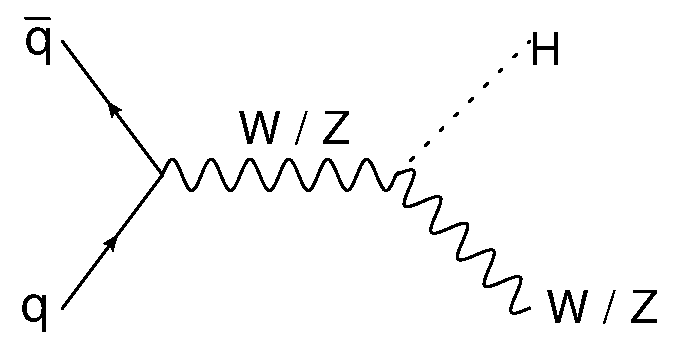
\includegraphics[width=1\linewidth]{T/FIGS/whzh}
					\end{minipage}
					\quad\quad
					\begin{minipage}[h]{0.4\linewidth}
						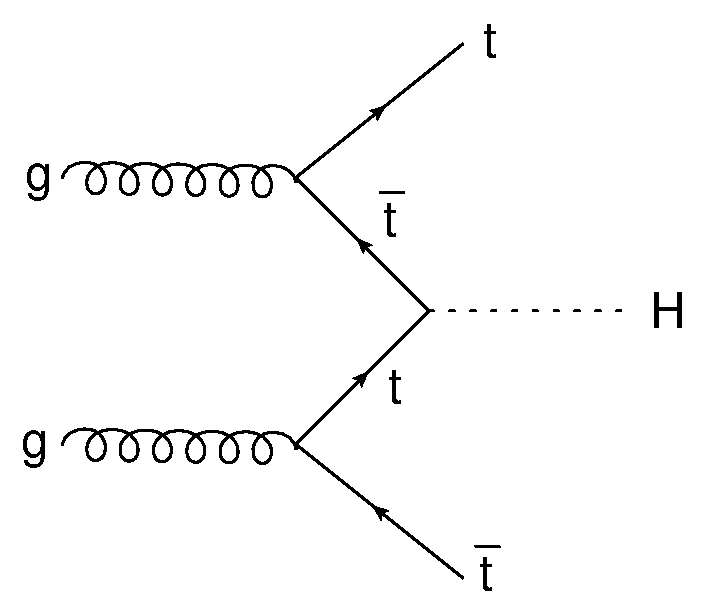
\includegraphics[width=1\linewidth]{T/FIGS/tth}
					\end{minipage}
				\caption{Lowest order Feynmann diagrams for gluon-gluon fusion (\ggF), $W/Z$ associated production ($WH/ZH$) and top anti-top associated production ($t\bar{t}H$).}
				\label{fig:higgsproddiag}
			\end{figure}


		\subsubsection{Gluon-gluon Fusion}

		The dominant production mechanism for the Higgs boson in hadron colliders is the \ggF\, production via in intermediate quark loop. The dynamics of this mechanism are controlled by strong interactions, thus calculations of QCD corrections are necessary for any accurate predictions, and have been computed up from next-to-leading order (NLO) to N$^3$LO for the \ggF process in recent years, along with the inclusion of Electro-Weak corrections in the cross section calculations \cite{LHCHiggsCS}.

	\subsection{Vector Boson Fusion}
	\label{t:VBF}

		Production of a Higgs boson from the fusion of vector bosons radiated from initial-state quarks is the second largest cross-section at the LHC, and is useful as a production mode due to topological characteristics which can distinguish the event from \ggF. In \VBFHBB, the characteristic topology is a pair of
		central \bjets forming the Higgs candidate, and two forward, close to the beam line VBF jets formed from remnants of the initially colliding protons as displayed in Figure \ref{fig:T:vbf}. In addition central jet activity is suppressed due to the lack of colour exchange between the colour single Higgs boson and the decay \bquarks \cite{VBF2004}.  These distinct features mean that while the cross section for VBF at a Higgs mass of $< 200$ GeV is dominated by \ggF, the easy to detect signature means the channel is a cornerstone of searches for the Higgs boson.

		\begin{figure}[h]
			\centering
			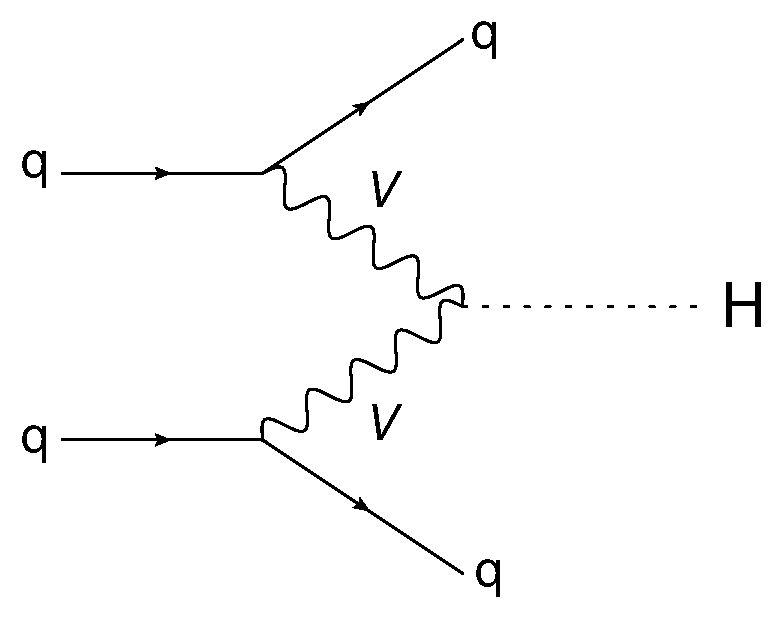
\includegraphics[width=0.4\linewidth]{T/FIGS/vbf}
			\caption{Feynmann diagram for the production of a Higgs boson via Vector Boson Fusion, where $q$ denotes any quark or antiquark}
			\label{fig:T:vbf}
		\end{figure}


	\subsection{Higgs Decay}

		The branching ratios for decays of the Higgs boson in the Standard Model have been extensively determined using Monte-Carlo event generators. As is to be expected, the relative cross-sections of the decay modes are strongly dependent on the mass of the Higgs boson, as highlighted in Figure \ref{fig:higgsbrlm}.

		\begin{figure}[h]
			\centering
			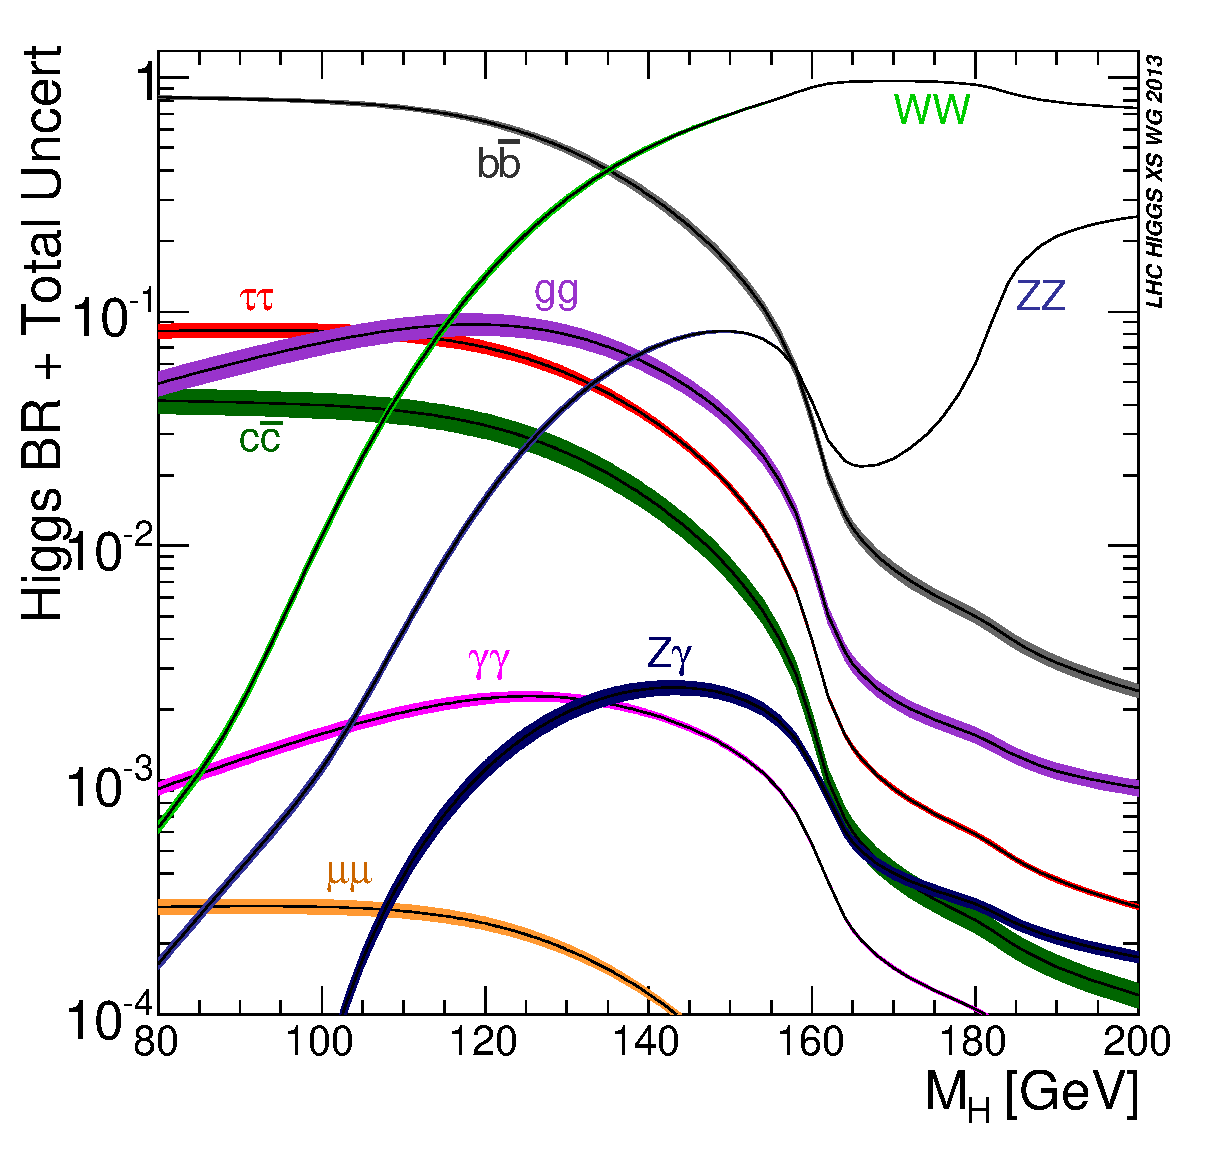
\includegraphics[width=0.5\linewidth]{T/FIGS/Higgs_BR_LM}
			\caption{Higgs decay branching ratios for the low mass region with their uncertainties \cite{LHCHiggsXS2013}.}
			\label{fig:higgsbrlm}
		\end{figure}

		\newpage
		While observations consistent with the Standard Model Higgs boson have been made for the $H\rightarrow \gamma\gamma$, $H\rightarrow ZZ$, $H\rightarrow W^+W^-$ and $H\rightarrow \tau^+\tau^-$ channels, observation of th $H\rightarrow bb$ decay channel is significantly hindered owing to the large background from multijet production in hadron collisions. Despite this, the topology of the VBF production mechanism makes it a viable option for observation of the  $b\bar{b}$ decay channel.

	\subsection{VBF Searches}

		Searches fo the \VBFHBB\, interaction look for a resonance in the invariant mass of a pair of jets containing \bquarks ($m_{bb}$) in events with the characteristic topology. This characteristic topology distinguishes the signal events from the multijet events that form the dominant background with a non-resonant $m_{bb}$ spectrum. An additional resonant background contribution to the \mbb spectrum is due to decay of a $Z$ boson to two jets in association with two jets.

		In the most recent searches for the Higgs boson produced via VBF, which this analysis emulates, the \VBFHBB\, events are indistinguishable from the \ggF\, events, and are separated using a multivariate boosted decision tree (BDT) analysis to refine the phase space to the most VBF sensitive BDT regions.


\endinput
